\documentclass{article}

\usepackage[
  paperwidth=841mm,
  paperheight=1188mm,
  margin=8mm
]{geometry}
\usepackage{iftex}
\ifLuaTeX
  \usepackage{fontspec}
  \usepackage{unicode-math}
  \IfFontExistsTF{Liberation Sans}
    {\setmainfont{Liberation Sans}}
    {\setmainfont{Arial}}
  \setmathfont{Latin Modern Math}
\else
  \usepackage[scaled]{helvet}
  \renewcommand{\familydefault}{\sfdefault}
\fi
\usepackage{xcolor}
\usepackage{graphicx}
\usepackage{tabularx}
\usepackage[most]{tcolorbox}
\usepackage{enumitem}
\usepackage{caption}
\usepackage{ragged2e}
\usepackage{amsmath}

\definecolor{ceaRed}{HTML}{E50019}
\definecolor{deepBlue}{HTML}{004C6D}
\definecolor{teal}{HTML}{009E73}
\definecolor{gold}{HTML}{D55E00}
\definecolor{lightGray}{HTML}{F5F5F5}
\definecolor{darkText}{HTML}{1B1B1B}

\pagestyle{empty}
\setlength{\parindent}{0pt}
\setlength{\parskip}{0.12em}
\captionsetup{font={small},labelformat=empty}
\setlist[itemize]{leftmargin=1.0em,itemsep=0.03em,topsep=0.02em}
\renewcommand{\arraystretch}{1.13}

\newcommand{\bodyfont}{\fontsize{21pt}{25pt}\selectfont}
\newcommand{\smallbody}{\fontsize{18pt}{22pt}\selectfont}
\newcommand{\reffont}{\fontsize{14pt}{17pt}\selectfont}
\newcommand{\headfont}{\fontsize{29pt}{34pt}\selectfont}
\newcommand{\titlefont}{\fontsize{47pt}{54pt}\selectfont}
\newcommand{\authorfont}{\fontsize{29pt}{34pt}\selectfont}
\newcommand{\institutefont}{\fontsize{23pt}{27pt}\selectfont}

\newtcolorbox{posterbox}[2][]{
  enhanced,
  width=\linewidth,
  colback=white,
  colframe=ceaRed,
  boxrule=2.4pt,
  arc=0pt,
  left=14pt,
  right=14pt,
  top=12pt,
  bottom=12pt,
  before skip=0pt,
  after skip=9pt,
  attach boxed title to top left={xshift=0pt,yshift=0pt},
  boxed title style={
    colback=ceaRed,
    colframe=ceaRed,
    boxrule=2.4pt,
    rounded corners=north,
    arc=16pt,
    sharp corners=south,
    left=14pt,
    right=14pt,
    top=7pt,
    bottom=7pt,
    width=\linewidth
  },
  title={\headfont\bfseries #2},
  coltitle=white,
  #1
}

\newcommand{\twocolrow}[4]{%
  \begin{minipage}[t]{0.492\linewidth}
    #1
  \end{minipage}
  \hfill
  \begin{minipage}[t]{0.492\linewidth}
    #2
  \end{minipage}
  #3#4%
}

\newcommand{\badge}[2]{%
  \begingroup
  \setlength{\fboxsep}{5pt}%
  \colorbox{#1!12}{\textcolor{#1}{\bfseries #2}}%
  \endgroup
}

\begin{document}
\bodyfont
\color{darkText}

\begin{tcolorbox}[
  enhanced,
  width=\linewidth,
  colback=white,
  colframe=white,
  borderline west={24pt}{-10pt}{ceaRed},
  boxrule=0pt,
  left=42pt,
  right=18pt,
  top=13pt,
  bottom=12pt,
  before skip=0pt,
  after skip=14pt
]
  \begin{minipage}[c]{0.16\linewidth}
    
\includegraphics[width=0.80\linewidth]{../MasterThesis/graphics/LOGO_CEA.png}
  \end{minipage}
  \hfill
  \begin{minipage}[c]{0.65\linewidth}
    \centering
    {\titlefont\bfseries Development of a Wavelet-Based Diffusion Surrogate Model\\
    for Two-Dimensional Rayleigh--Taylor Instability\par}
    \vspace{0.55em}
    {\authorfont\bfseries Samuel Chapuis\par}
    \vspace{0.25em}
    {\institutefont CEA Bruyeres-le-Chatel -- Materiaux en conditions extremes\par}
  \end{minipage}
  \hfill
  \begin{minipage}[c]{0.15\linewidth}
    \raggedleft
    {\headfont\bfseries 2025--2026}
  \end{minipage}
\end{tcolorbox}

\begin{posterbox}[height=150mm,valign=top]{Physical Problem}
  \begin{minipage}[t]{0.54\linewidth}
    \vspace{0pt}
    \badge{deepBlue}{Context} \quad Direct Numerical Simulations of Rayleigh--Taylor instability provide high-fidelity density fields, but their cost limits the number of available realizations.
    \begin{itemize}
      \item RTI occurs when a dense fluid is accelerated by a lighter one; perturbations grow into bubbles, spikes and turbulent mixing.
      \item The flow is nonlinear and strongly multi-scale: large coherent structures coexist with sharp interfaces and localized fluctuations.
      \item Goal: learn the distribution of two-dimensional RTI density fields and generate new physically plausible samples.
    \end{itemize}
  \end{minipage}
  \hfill
  \begin{minipage}[t]{0.45\linewidth}
    \vspace{0pt}
    \centering
    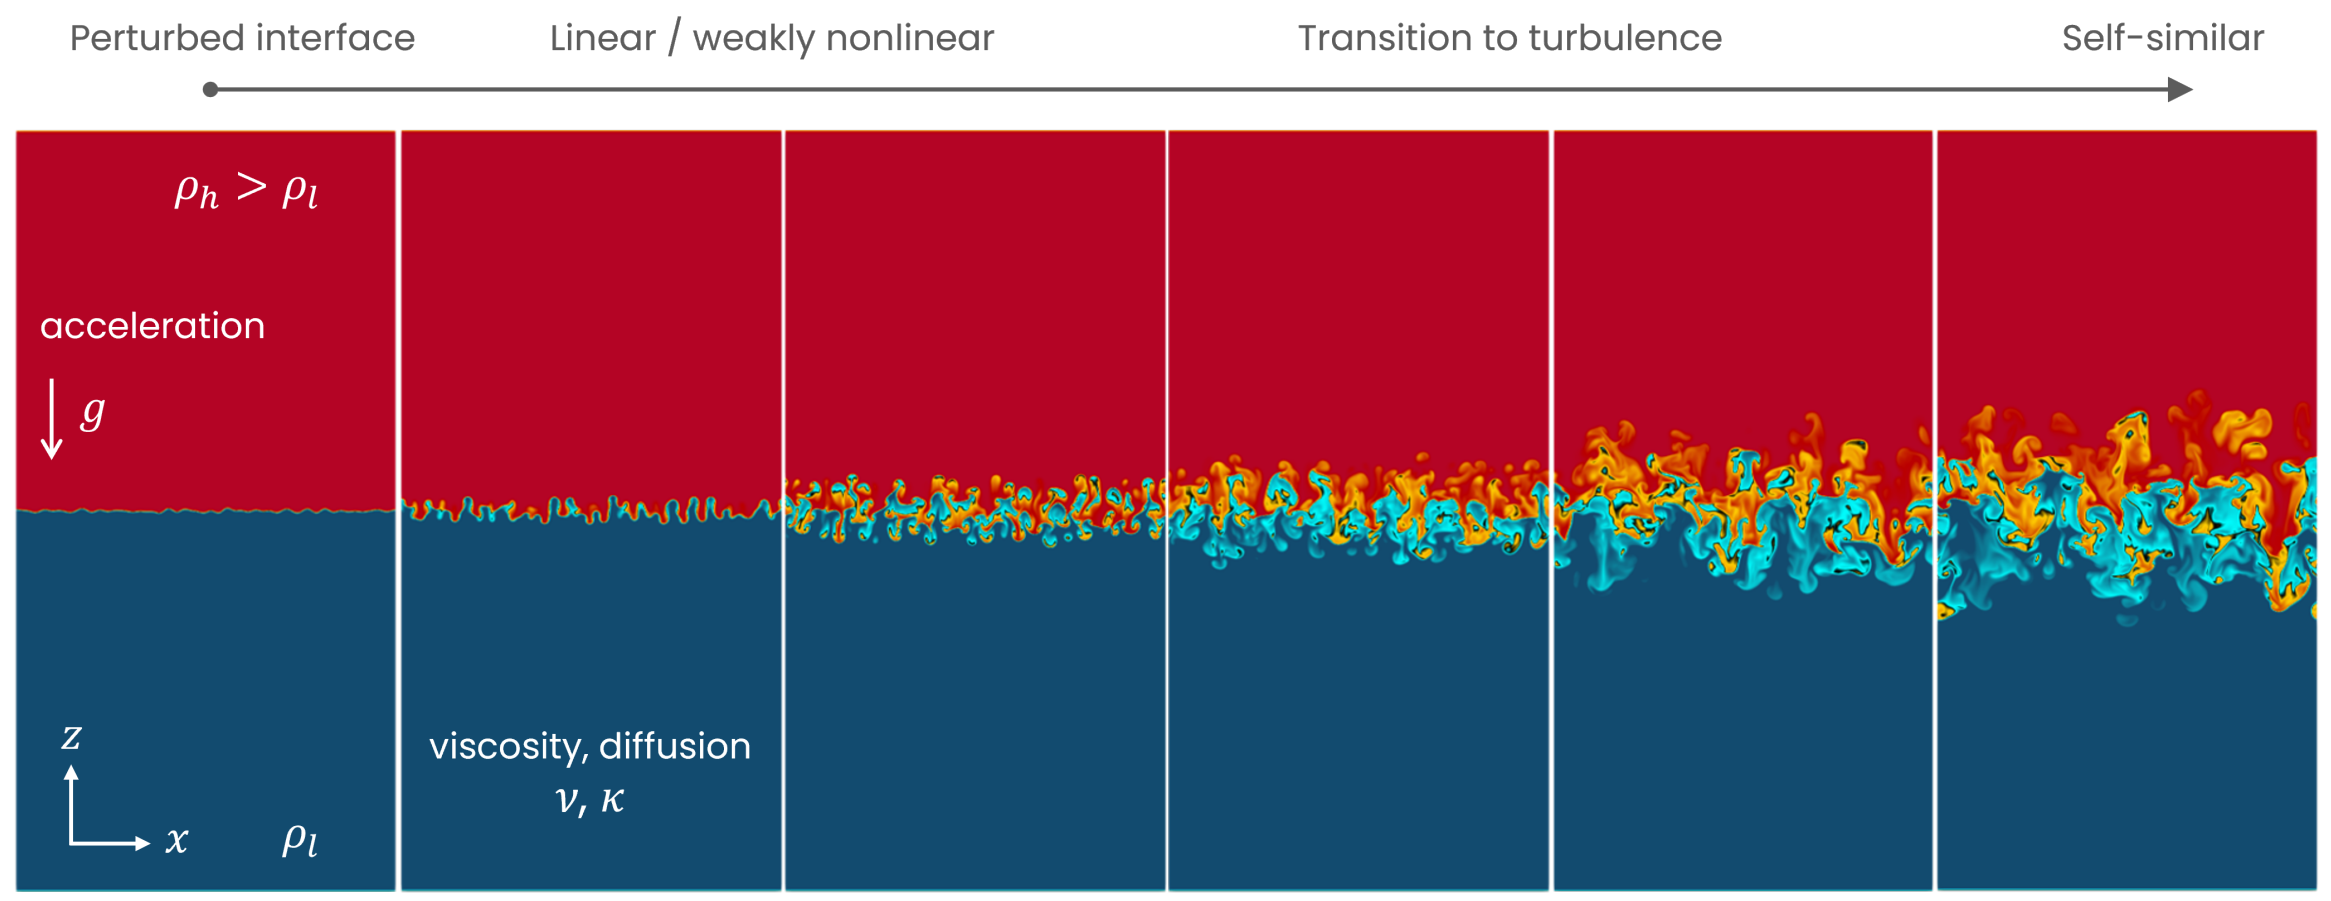
\includegraphics[height=130mm,keepaspectratio]{figures/RTI-Sebastien_Thevenin.png}
    \captionof{figure}{Temporal evolution of a Rayleigh--Taylor density field from DNS.}
  \end{minipage}
\end{posterbox}

\begin{minipage}[t]{0.492\linewidth}
\begin{posterbox}[height=166mm,valign=top]{Multi-resolution Representation}
  \begin{itemize}
    \item Fourier modes are natural for periodic flows, but they are global.
    \item Wavelets localize information both in space and scale.
    \item A 2D DWT separates approximation coefficients $c_A$ from details $c_H,c_V,c_D$.
    \item This gives a compact hierarchy for interfaces, vortices and mixing layers.
  \end{itemize}
  \vspace{0.35em}
  \centering
  
\includegraphics[width=0.88\linewidth,height=115mm,keepaspectratio]{figures/wavelet_decomposition.png}
\end{posterbox}
\end{minipage}
\hfill
\begin{minipage}[t]{0.492\linewidth}
\begin{posterbox}[height=166mm,valign=top]{Score-Based Diffusion Models}
  A diffusion model learns a reverse denoising process:
  \[
    x_t=\sqrt{\bar\alpha_t}x_0+\sqrt{1-\bar\alpha_t}\epsilon,
    \qquad
    \epsilon_\theta(x_t,t)\approx\epsilon .
  \]
  The trained U-Net maps Gaussian noise back toward the RTI data distribution.
  \vspace{0.35em}
  \centering
  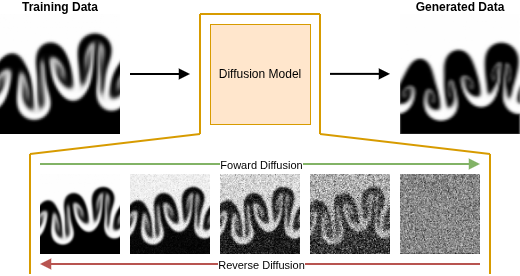
\includegraphics[width=0.82\linewidth,height=120mm,keepaspectratio]{figures/fast_diffusion.png}
\end{posterbox}
\end{minipage}


% \begin{posterbox}[height=150mm,valign=top]{Physical Problem}
%   \begin{minipage}[t]{0.54\linewidth}
%     \vspace{0pt}
%     \badge{deepBlue}{Context} \quad Direct Numerical Simulations of Rayleigh--Taylor instability provide high-fidelity density fields, but their cost limits the number of available realizations.
%     \begin{itemize}
%       \item RTI occurs when a dense fluid is accelerated by a lighter one; perturbations grow into bubbles, spikes and turbulent mixing.
%       \item The flow is nonlinear and strongly multi-scale: large coherent structures coexist with sharp interfaces and localized fluctuations.
%       \item Goal: learn the distribution of two-dimensional RTI density fields and generate new physically plausible samples.
%     \end{itemize}
%   \end{minipage}
%   \hfill
%   \begin{minipage}[t]{0.45\linewidth}
%     \vspace{0pt}
%     \centering
%     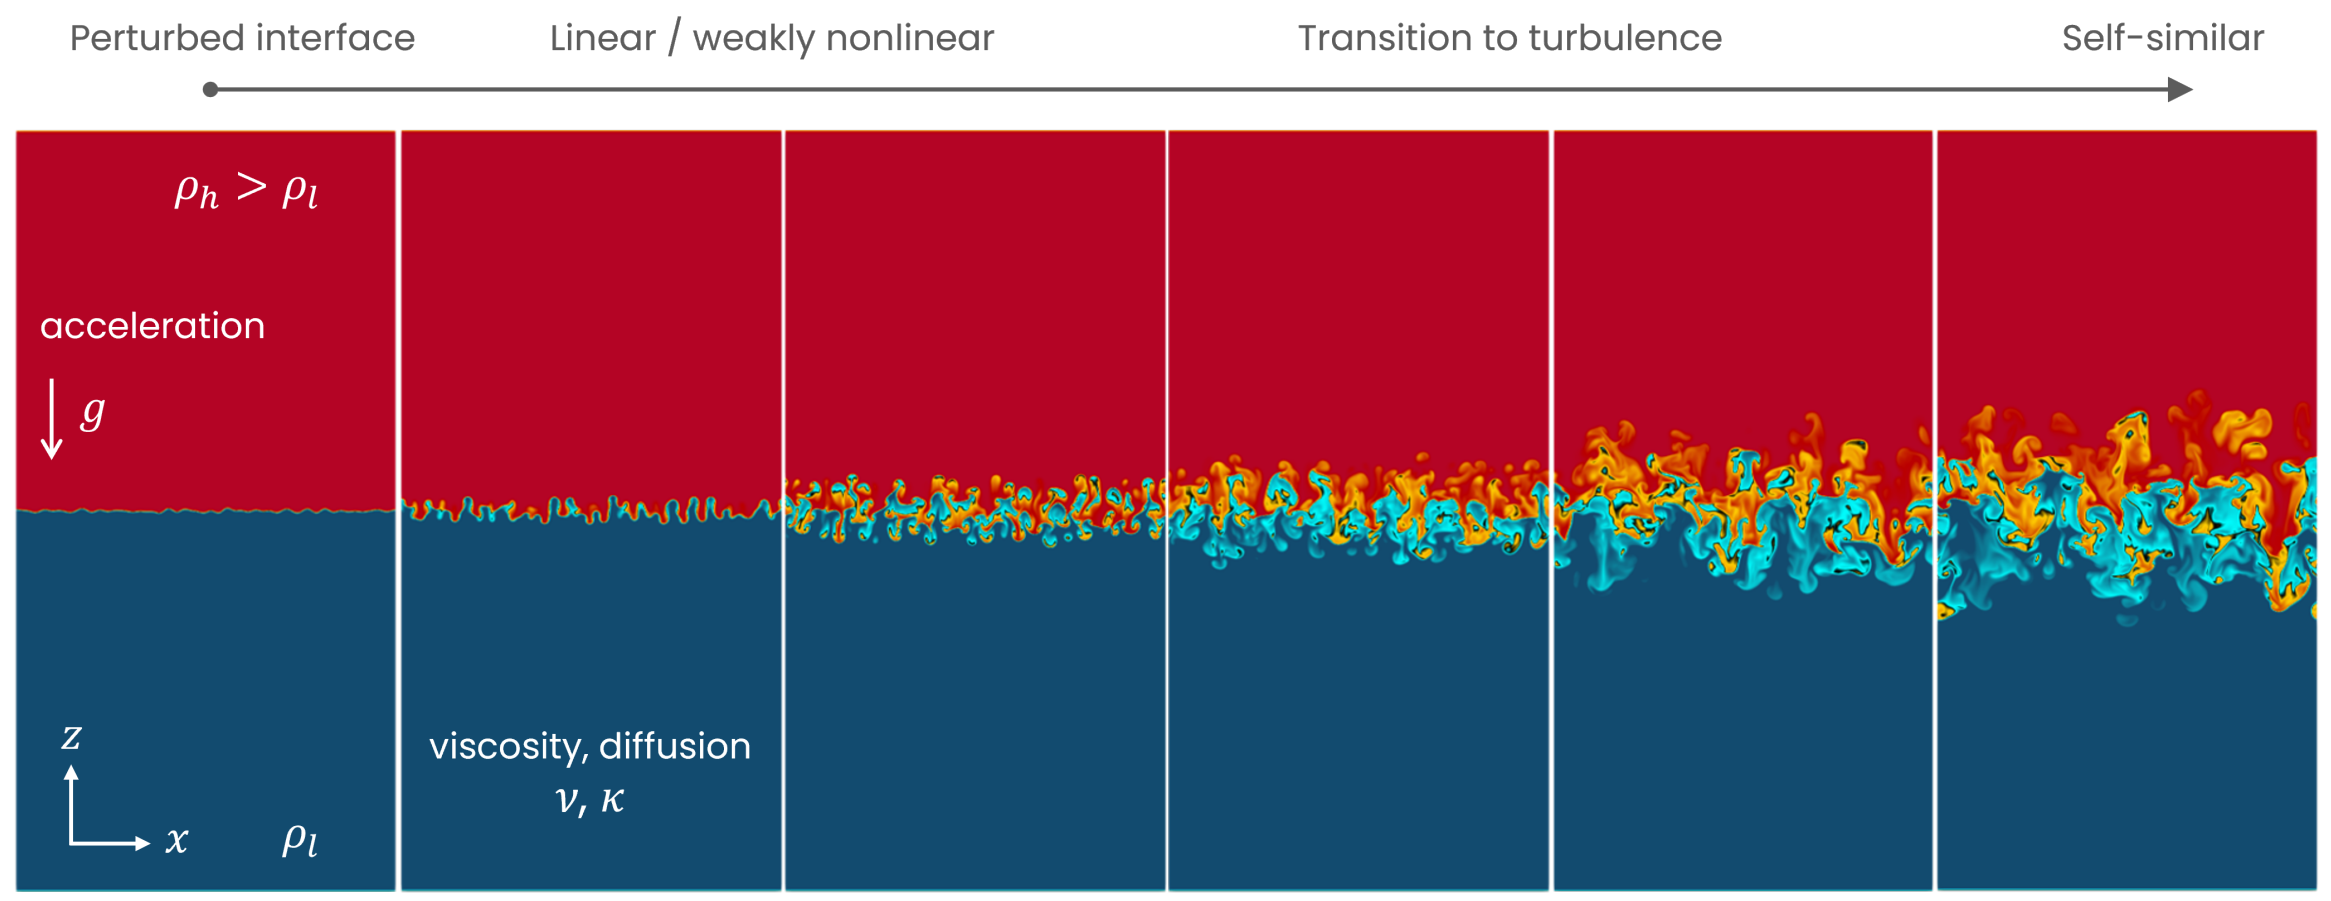
\includegraphics[height=130mm,keepaspectratio]{figures/RTI-Sebastien_Thevenin.png}
%     \captionof{figure}{Temporal evolution of a Rayleigh--Taylor density field from DNS.}
%   \end{minipage}
% \end{posterbox}
\vspace{8px}
\begin{posterbox}[height=170mm,valign=top]{Hierarchical Wavelet Diffusion}
  \begin{minipage}[t]{0.54\linewidth}
    \vspace{0pt}
    \badge{teal}{Coarse prior} \quad The approximation coefficients $c_A$ are generated first, capturing the main vertical organization of the mixing zone.
    \begin{itemize}
      \item Train a DDPM on the low-resolution $c_A$ fields.
      \item Sample new $c_A$ fields from the learned distribution.
    \end{itemize}
    \vspace{0.3em}
    \badge{gold}{Conditional details} \quad The detail coefficients $c_H,c_V,c_D$ are generated conditionally on the coarse content, allowing for scale-aware synthesis.
    \begin{itemize}
      \item Train three conditional DDPMs for horizontal, vertical and diagonal details.
      \item Sample new detail coefficients conditioned on the generated $c_A$ fields.
    \end{itemize}
  \end{minipage}
  \hfill
  \begin{minipage}[t]{0.45\linewidth}
    \vspace{0pt}
    \centering
    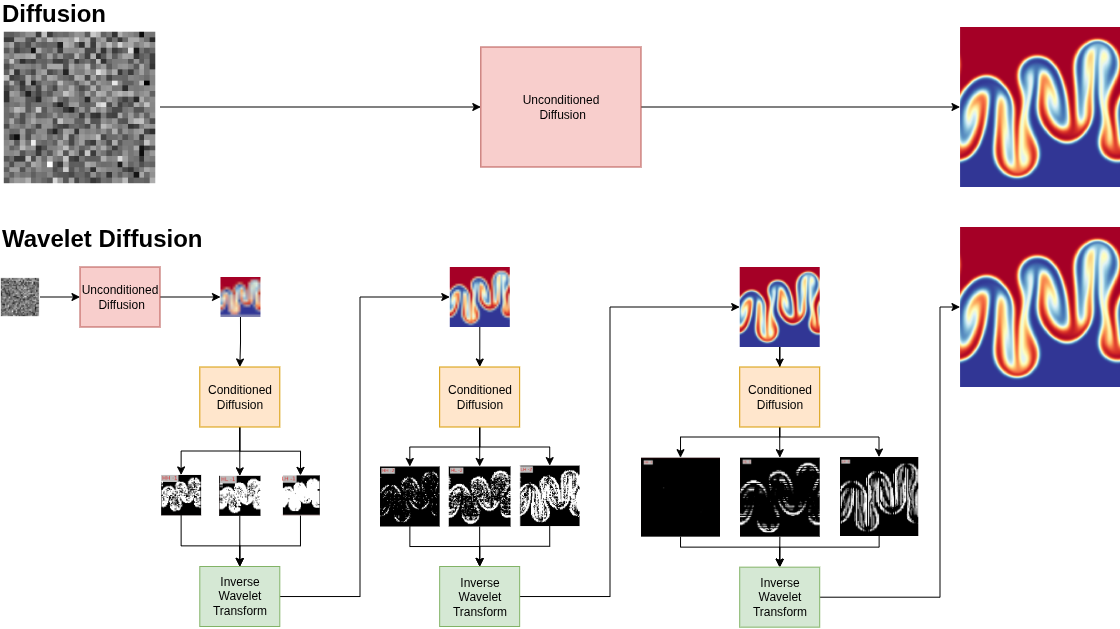
\includegraphics[width=\linewidth,height=150mm,keepaspectratio]{figures/WaveletDiffusion.png}
    \captionof{figure}{Hierarchical wavelet diffusion: coarse approximation coefficients are generated first, then detail coefficients are synthesized conditionally.}
  \end{minipage}
\end{posterbox}


% \vspace{3px}
\begin{minipage}[t]{0.37\linewidth}
\begin{posterbox}[height=298mm,valign=top]{Experimental Setup}
  \smallbody
  \begin{tabularx}{\linewidth}{>{\bfseries}p{0.31\linewidth}X}
    Data & DNS Rayleigh--Taylor density snapshots, preprocessed as $64\times64$ images. \\
    Splits & Training, validation and test tensors; validation contains 6528 fields. \\
    Augmentation & Horizontal periodic translations and horizontal reflections. \\
    Wavelets & 2D DWT, Daubechies-1 basis, levels $j=3,2,1$. \\
    Models & Baseline DDPM in image space; conditional DDPMs for wavelet details. \\
    Metrics & FID, domain-adapted PhyFID, vertical density profiles and fluctuation spectra. \\
  \end{tabularx}
  \vspace{0.45em}
  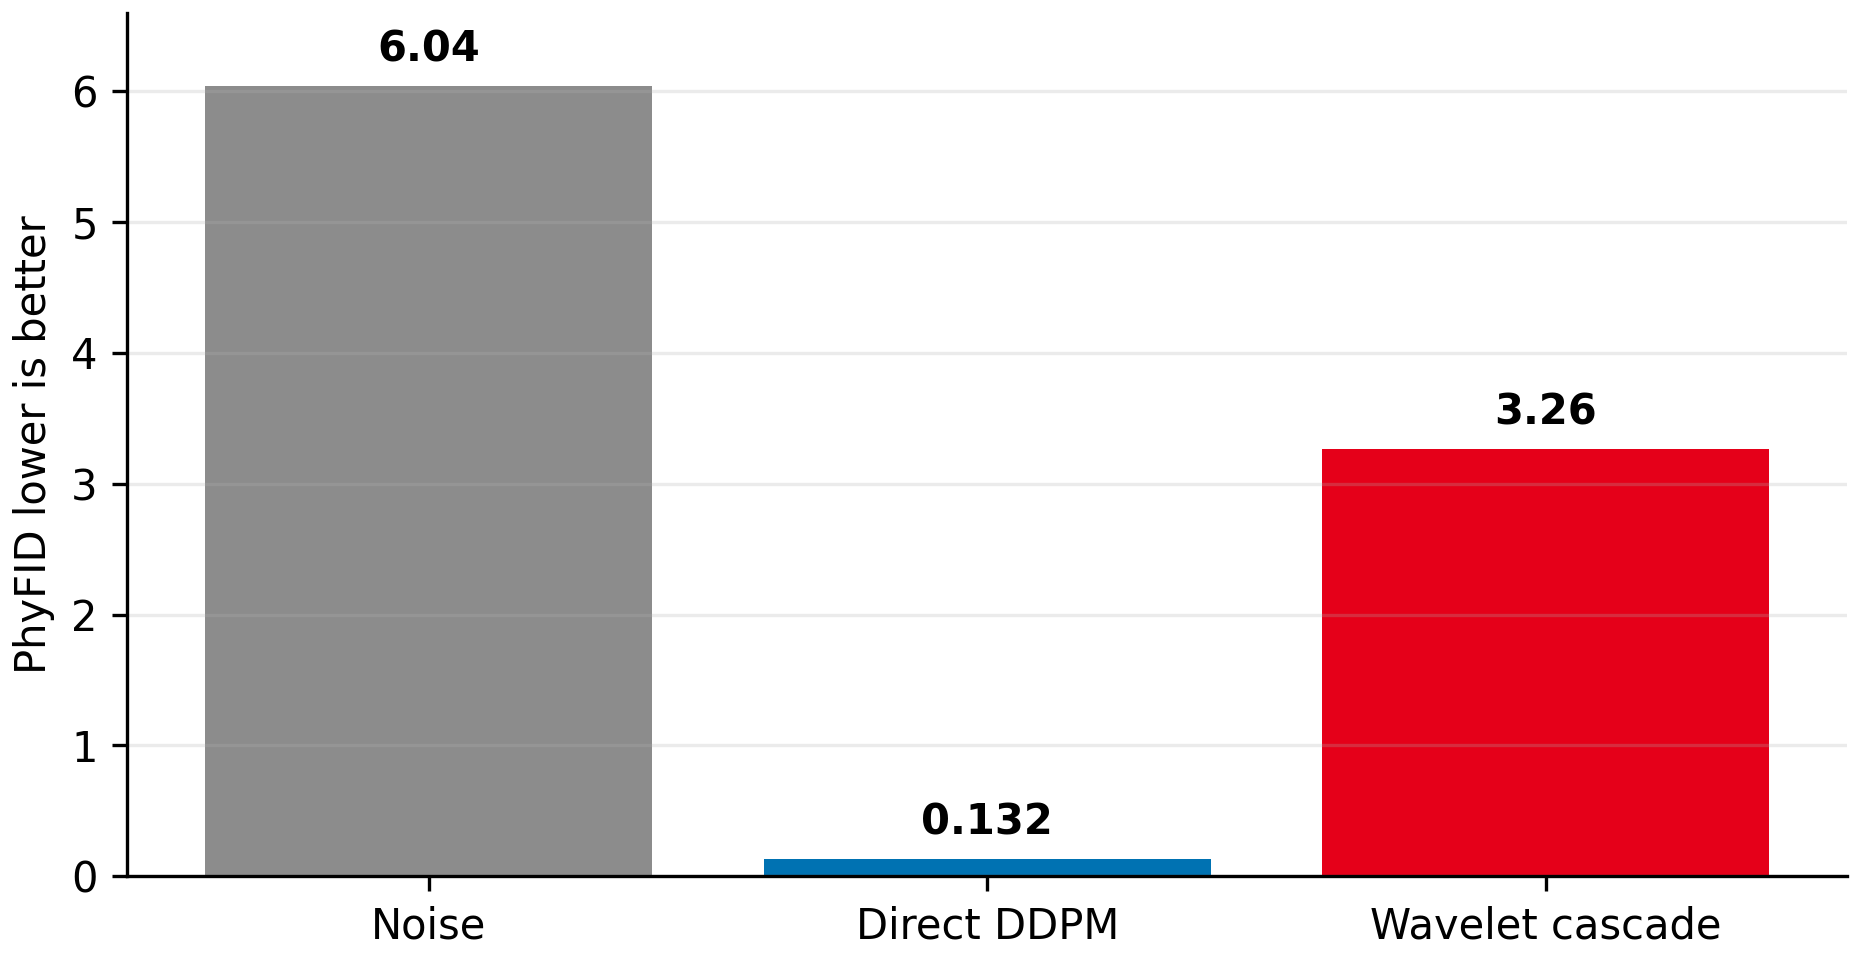
\includegraphics[width=\linewidth,height=85mm,keepaspectratio]{figures/phyfid_summary.png}
\end{posterbox}
\end{minipage}
\hfill
\begin{minipage}[t]{0.612\linewidth}
\begin{posterbox}[height=298mm,valign=top]{Results}
  \begin{minipage}[t]{0.55\linewidth}
    \centering
    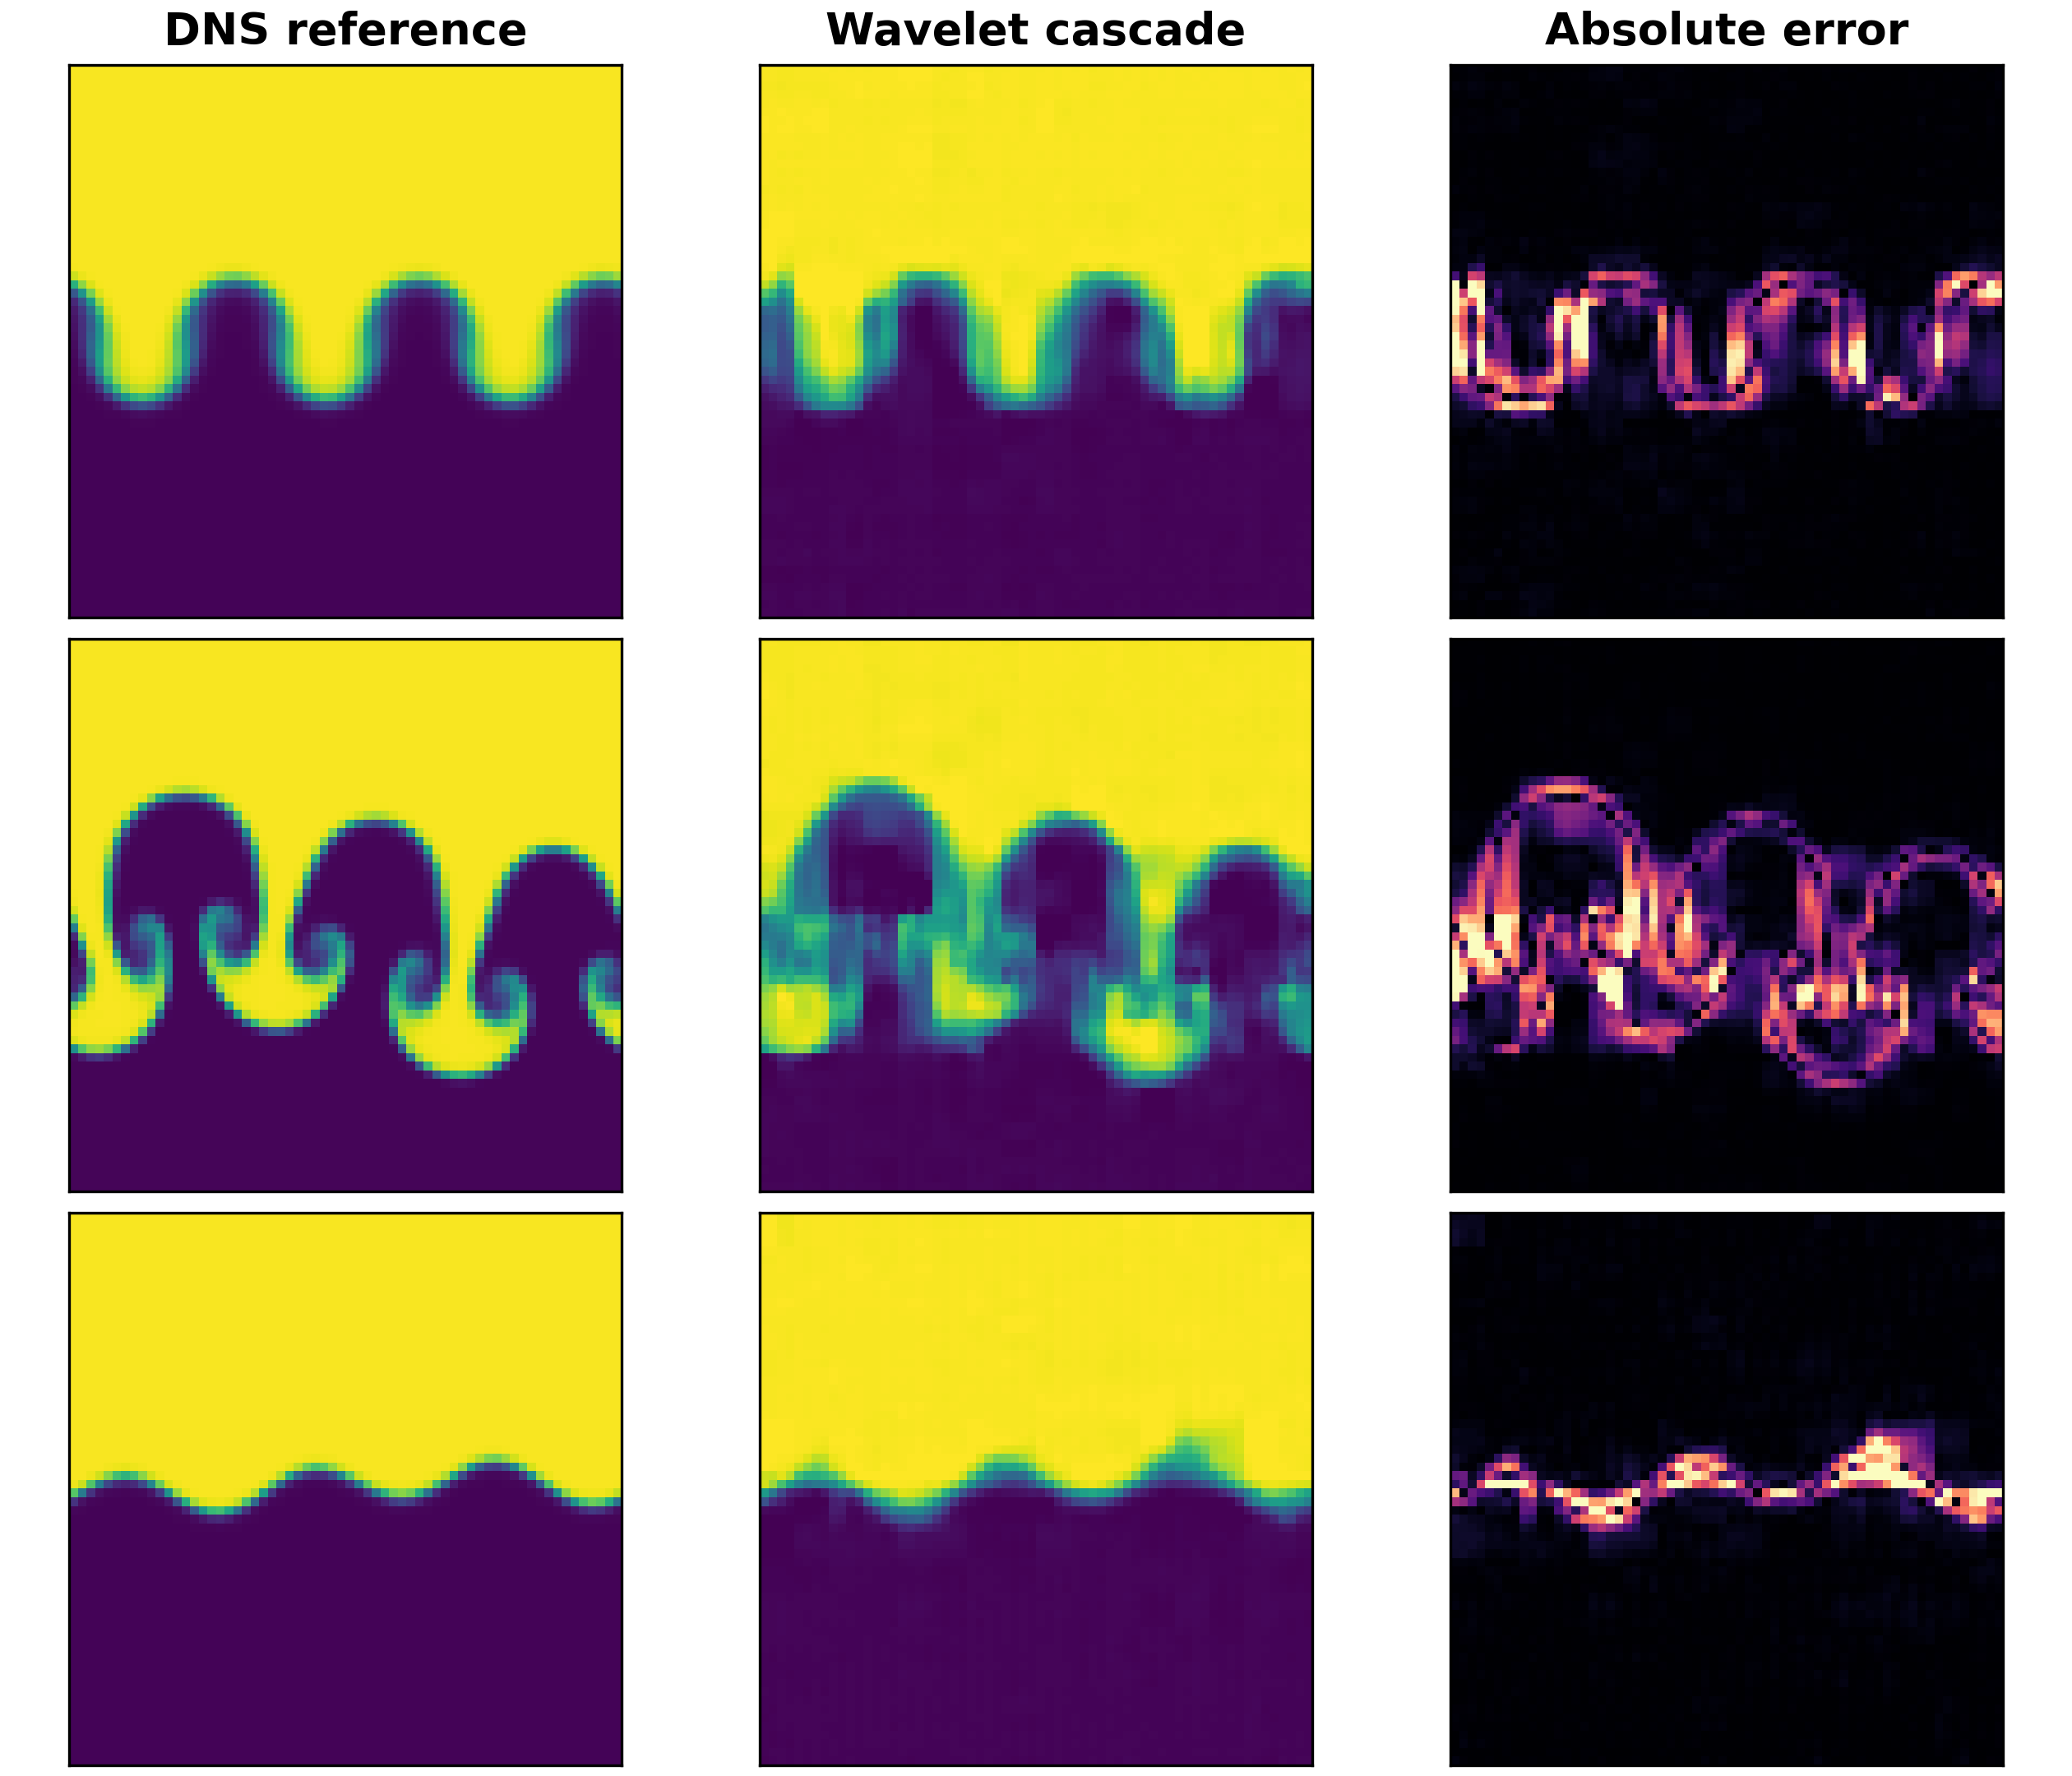
\includegraphics[width=\linewidth,height=220mm,keepaspectratio]{figures/cascade_reconstruction_comparison.png}
  \end{minipage}
  \hfill
  \begin{minipage}[t]{0.42\linewidth}
    \centering
    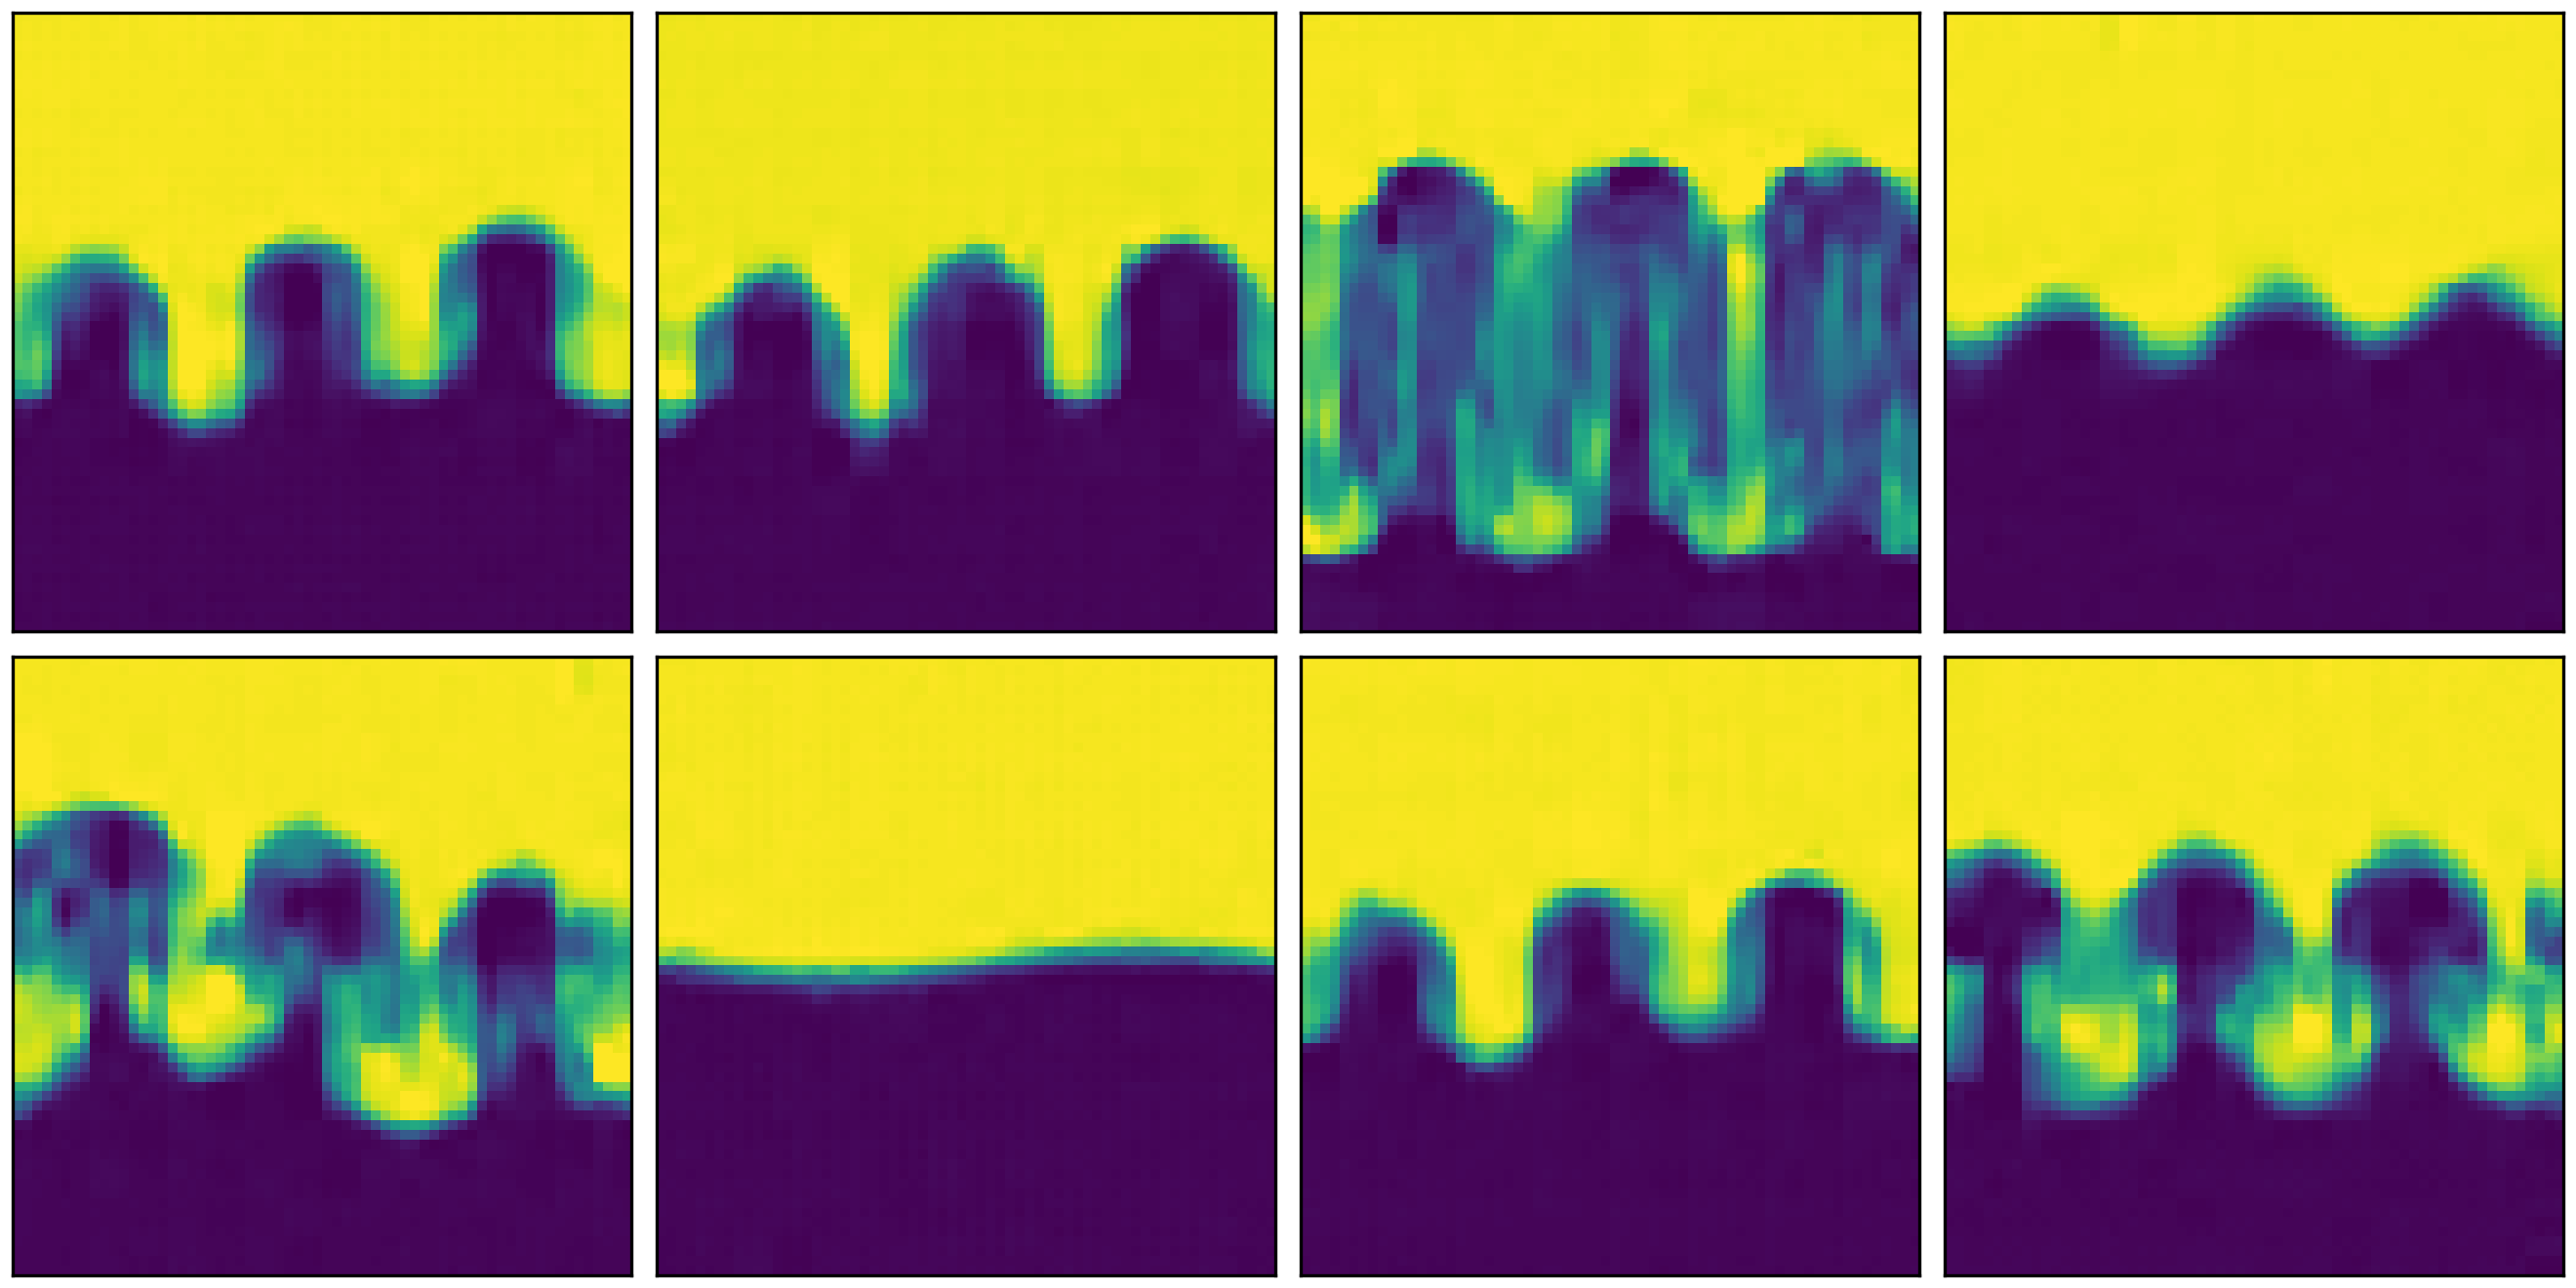
\includegraphics[width=\linewidth,height=95mm,keepaspectratio]{figures/cascade_generated_samples.png}
    \vspace{0.3em}
    \begin{itemize}
      \item Direct DDPM captures the main vertical organization of the mixing zone and gives the best current PhyFID.
      \item Wavelet cascade preserves the low-frequency morphology but produces rougher fine-scale details.
      \item The coefficient-space formulation is useful diagnostically: artifacts can be assigned to specific scales.
    \end{itemize}
  \end{minipage}
\end{posterbox}
\end{minipage}

\vspace{10px}
\begin{minipage}[t]{0.492\linewidth}
\begin{posterbox}[height=82mm,valign=top]{References}
  \reffont
  Zhou, Y. (2017). Rayleigh--Taylor and Richtmyer--Meshkov instability induced flow, turbulence, and mixing. \emph{Physics Reports}.\\
  Ho, J., Jain, A., Abbeel, P. (2020). Denoising diffusion probabilistic models. \emph{NeurIPS}.\\
  Song, Y. et al. (2021). Score-based generative modeling through stochastic differential equations. \emph{ICLR}.\\
  Mallat, S. (2009). \emph{A Wavelet Tour of Signal Processing}.
\end{posterbox}
\end{minipage}
\hfill
\begin{minipage}[t]{0.492\linewidth}
\begin{posterbox}[height=82mm,valign=top]{Future Work}
  \begin{minipage}[t]{0.58\linewidth}
    \begin{itemize}
      \item Complete quantitative evaluation of the wavelet cascade.
      \item Test alternative wavelet families and decomposition depths.
      \item Improve multi-level conditioning from coarse to fine scales.
      \item Scale to larger datasets and higher resolutions.
      \item Use conditional generation for rare RTI regimes and inverse design.
    \end{itemize}
  \end{minipage}
  \hfill
  \begin{minipage}[t]{0.38\linewidth}
    \centering
    \badge{teal}{coarse prior}\\[0.6em]
    $\Downarrow$\\[0.3em]
    \badge{gold}{conditional details}\\[0.6em]
    $\Downarrow$\\[0.3em]
    \badge{ceaRed}{scale-aware samples}
  \end{minipage}
\end{posterbox}
\end{minipage}

\vspace{10px}
\begin{tcolorbox}[
  width=\linewidth,
  colback=ceaRed,
  colframe=ceaRed,
  boxrule=2.4pt,
  arc=0pt,
  left=18pt,
  right=18pt,
  top=10pt,
  bottom=10pt,
  before skip=0pt,
  after skip=0pt
]
  {\headfont\bfseries\color{white} Key message: wavelet diffusion introduces a physically interpretable multi-scale inductive bias, but the direct image-space DDPM remains the stronger baseline at the present stage.}
\end{tcolorbox}

\end{document}
